% Tizedik és tizenegyedik előadás

\chapter{I/O rendszer}

A CPU-t és a perifériákat összekötő egységet hívjuk I/O egységnek.
Például egy billentyűzet csatlakozásánál az alaplapi USB vezérlő számít I/O egységnek.

\section{Fejlődésük}
\begin{enumerate}
    \item A CPU közvetlenül vezérli a perifériát (megszakítás nélküli programozott IO - wait for flag)
    \item Egy I/O modul kerül kialakításra
    \begin{itemize}
        \item megszakítás nélkül, wait for flag
        \item megszakításos vezérlés
    \end{itemize}
    \item DMA segítségével közvetlen hozzáférés a perifériához
    \item IO csatorna - lassabb perifériák számára. IO-ra specializált utasításkészlettel rendelkezik és a központi operatív tárat használja
    \item IO processzor - az IO csatorna továbbfejlesztése, saját működésre képes egység, saját memóriával
\end{enumerate}

\section{Programozott I/O}
Működés szerint megkülönböztetünk lekérdezéses és megszakításos I/O-t, címzés szerint pedig különálló címterű és memóriában leképzett címterű I/O-t.

\subsection{Lekérdezéses és megszakításos vezérlések}
A megszakítás nélküli vezérlés nagy hátránya, hogy az utasítás kiküldése után a CPU egy ciklusban várakozik a periféria válaszára, és amíg ez meg nem érkezett, blokkolta a további műveleteket.
Ezért jelentek meg a megszakításrendszerek, a processzor az utasítás kiadása után más feladatokkal foglalkozott, majd az IO egység megszakítással jelzi a művelet befejezését.
Következmény, hogy nő a teljesítmény.

\subsection{Különálló címterű IO}
A különálló I/O címtérnél a CPU két címteret lát: az I/O és az operatív tár.
A két címzés közös buszt használ, ezért külön utasítások tartoznak az IO műveletekhez.
Következmény, hogy lehet azonos egy memória és egy IO cím.
Ehhez kellenek busz vezérlő jelek (M/IO jel) és speciális utasítások (pl. IN X, OUT X).
\begin{figure}[H]
    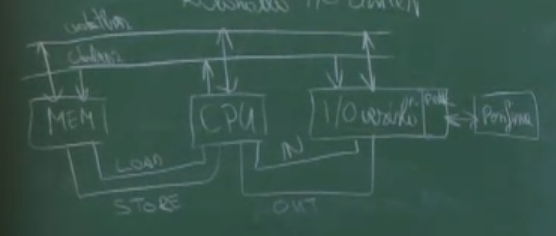
\includegraphics[width=0.5\textwidth]{cimzes}
    \centering
    \caption{A memória és IO címzés}
    \label{fig:cimzes}
\end{figure}
\subsubsection{Értékelés}
A különálló címterű I/O előnye az egyszerű megvalósítás, viszont terheli a CPU-t és plusz utasításokra van szükség.

\subsection{Memóriában leképzett IO}
Ekkor a memória egy része az IO egységeknek fenntartott, az adatok olvasása és írása LOAD/STORE utasításokkal történik.
Az IO vezérlő ilyenkor hozzáfér a rendszerbuszhoz, gyorsabb az átvitel.
\begin{figure}[H]
    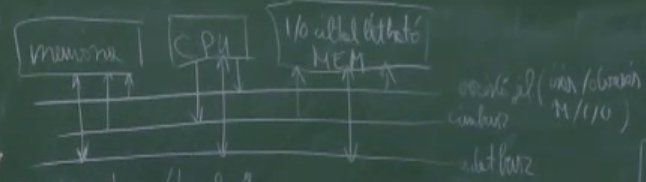
\includegraphics[width=0.5\textwidth]{cimzes2}
    \centering
    \caption{Memóriában leképzett IO címzése}
    \label{fig:cimzes2}
\end{figure}
Példa: a grafikus vezérlő megengedi a processzor számára, hogy közvetlenül címezze a framebuffert, ami a képernyőn adott pillanatban megjelenő kép adatait tartalmazza.


\subsection{Az I/O vezérlő}
Az IO vezérlő egy kártyán helyezkedik el, ezen a kártyán vannak az IO portok (a rendszerbusz és a periféria közötti csatlakozási pont).
Az IO port egy egyedi azonosítóval ellátott eszköz, saját címe van és legalább egy adatregisztert tartalmaz.
A vezérlő tartalmaz:
\begin{itemize}
    \item parancsregisztert, ide írja a CPU a kívánságait
    \item adatregisztereket (data input és output)
    \item állapotregisztert - állapotinformációkat közöl a perifériáról, minden bitje mást jelent. Ilyen állapotok pl.:
    \begin{itemize}
        \item megszakítás kérés
        \item ready
        \item foglalt (busy)
    \end{itemize}
    \item jelenlét ellenőrző regiszter - megmondja, hogy van-e eszköz kapcsolva az I/O portra
    \item eszköz tulajdonságait tartalmazó regiszter (plug and play)
\end{itemize}
Bonyolultabb perifériák esetén egyes funkciókhoz akár több regiszter is tartozhat.

\subsection{Működése}
Az IO működését átviteli módszerek alapján két csoportra osztjuk:
\begin{itemize}
    \item feltétel nélküli adatátvitel (direkt programozott)
    \item feltételes adatátvitel
\end{itemize}
Feltétel nélküli adatátvitelnél a perifériának mindig adatátvitelre alkalmas állapotban kell lennie.
Ellenőrzésre sem az átvitel előtt, sem után nincs szükség és szinkronizálás sincs a CPU és a periféria között.
Ilyen működésű pl. a kijelző, a processzor nem foglalkozik azzal, ha a monitor pixelhibás.
Hátránya, hogy nincs visszacsatolás.

Feltételes adatátvitelnél valamilyen feltétel teljesülése esetén valósul meg az adatátvitel.
Ilyen pl. a nyomtatók.
Ennek a két csoportja a lekérdezéses és a megszakításos adatátvitel.
Lekérdezésesnél a processzor folyamatosan figyeli az állapotregiszter tartalmát.
Fejlettebb változata a megszakításos működés, ennél csak az IO regiszter által küldött megszakításnál kérdezi le az állapotregisztert és a megszakítás kiszolgálása eredményezi az adatátvitelt.
Ez a módszer viszont még mindig lassú és sok megszakítással jár, mivel mindent a CPU vezérel.
Ennek a kiküszöbölésére találták ki a Direct Memory Access-t (DMA).

\section{DMA}
Adatátvitel szerint csoportosítjuk:
\begin{itemize}
    \item blokkos
    \item cikluslopásos
\end{itemize}

A DMA-t alkalmazzák:
\begin{itemize}
    \item nagy mennyiségű adat átvitelénél (általában blokkos átvitel)
    \item gyors perifériáknál
\end{itemize}
Az adatátvitel a CPU közreműködése nélkül történik.
A DMA mellett megmarad az IO vezérlő is, ami a lassú perifériák számára biztosítja az adatátvitelt.
\begin{figure}[H]
    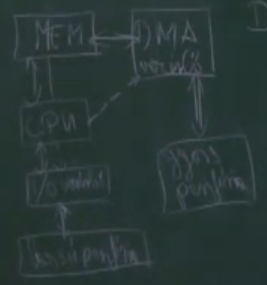
\includegraphics[width=0.5\textwidth]{dma}
    \centering
    \caption{A DMA felépítése}
    \label{fig:dma}
\end{figure}
A DMA lényege, hogy viszonylag kis mértékű komplexitás növekedés segítségével tehermentesíthető a CPU és megvalósítható a közvetlen adatátvitel.
A DMA a processzor helyett végzi a perifériákról a memóriába beolvasást.
A DMA vezérlő tulajdonságai:
\begin{itemize}
    \item címet kell tudnia generálni (a memória rekeszek címzéséhez)
    \item buszvezérlési funkciókat kell megvalósítania
\end{itemize}
Ezt a módszert nevezzük közvetlen tárhozzáférésnek.
Előnye, hogy jóval kevesebb megszakítás szükséges.

\subsection{A DMA vezérlő}
A DMA saját regiszterekkel rendelkezik, pl. IO cím, IO data, DC, saját belső vezérlővel és rejtett regiszterekel is felszerelt.
Műdödési lépései:
\begin{enumerate}
    \item felparaméterezés: a processzor betölti a szükséges adatokat a DMA-ba (ez programozott IO-val történik). Az átadott paraméterek: írási/olvasási műveletet kell végrehajtani (irány), az IO egység címe, a memóriacím kezdőértéke (IO address regiszter), átvivendő adat jellege (pl. byte, félszó, szó), olvasandó/írandó egységek száma (DC-be), átvitel módja (blokkos/cikluslopásos), DMA csatornáihoz rendelt prioritási érték, résztvevő egységek (pl. mem-mem, IO-mem, IO-IO)
    \item második lépésbel eltér a blokkos adatátvitel és a cikluslopásos:
    \begin{itemize}
        \item blokkos átvitel esetén az átvitel idejére a DMA lefoglalja a buszt, a paraméterek bekerülnek a DMA regisztereibe
        \item cikluslopásos átvitelnél nem a teljes átvitelre foglalja le a buszt, csak bizonyos időtartamokra (olyan ciklusoknál, amikor a CPU nem használja a rendszerbuszt, azaz decode és execute fázisokban - ezek a DMA töréspontok). Ezt kevesebb adat esetén használják.
    \end{itemize}
    \item a DMA megszakítás kérést küld a processzornak (DMA request)
    \item a CPU egy DMA acknowledge jelzést küld a DMA vezérlőnek
    \item az IO címregiszterbe a DMA betölti az első címet, majd kiteszi a címbuszra
    \item beolvassa a perifériából az információt az IO data regiszterbe
    \item az IO data regiszterből betölti az operatív tárba az adatot
    \item dekrementálja a Data Counter regiszter tartalmát és megnézi, hogy nulla-e
    \item ha nulla, küld egy megszakítást a processzornak, amiben jelzi, hogy befejeződött az átvitel. Ha nem nulla, inkrementálja a címregisztert és újrakezdi a beolvasást.
    \item a processzor ellenőrzi az adatátvitelt és visszaveszi a vezérlést, megszünteti a buszhasználat engedélyezését
\end{enumerate}

A cikluslopásos végrehajtást ma már nem nagyon használják, mivel a futószalag és a párhuzamos végrehajtás miatt a buszrendszer gyakorlatilag folyamatosan használatban van.

\section{I/O csatorna}
Típusai:
\begin{itemize}
    \item szelektor csatorna
    \item multiplexer csatorna
\end{itemize}

